\label{fs-formalism}

In this section, we introduce a formal model of a distributed stream processing system. After that, we define the notions of delivery guarantees in a regular way. We demonstrate that in a general case, non-deterministic systems must save results of non-commutative operations before output delivery. It is illustrated how state-of-the-art stream processing systems fit the requirements that we formulate.

\subsection{Preliminaries}
% In this section, we remind the main concepts of stream processing, that we use further in this paper. 

A distributed stream processing system is a shared-nothing distributed runtime, that can handle a potentially infinite sequence of input items. Each item can be transformed several times before the final result is released from the system. Output elements may depend on multiple input ones. Elements can be processed one-by-one or grouped into small input sets, usually called {\em micro-batches}. 

A user specifies required stream processing with a {\em logical graph}. Vertices of this graph represent operations and edges determine the data flow between tasks. A processing system maps the logical graph to a {\em physical} graph that is used to control actual distributed execution. Commonly, each logical operation is mapped to several physical tasks that are deployed to a cluster of computational units connected through a network. Each operation may be {\em stateless} or {\em stateful}. A system is usually responsible for state management in order to prevent inconsistencies.

An input element has {\em entered} if the system is aware of this element since that moment and takes some responsibility for its processing. 
This concept can be implemented differently. 
For example,
 an  element has been entered when  it  has arrived at {\em Source} vertex in Flink, while   
an element enters, when it is read or received by an input agent also called  {\em Source}   in Spark Streaming.

An output element has {\em left} the system if the element has been released to a consumer. 
Since that time, the system cannot observe it anymore. This concept can also be implemented differently in various systems. For instance, in Spark Streaming element leaves when it is pushed to output operation, e.g., written to HDFS or file. In Flink, an element is delivered to end-user when it leaves from {\em Sink} vertex.   

It is important to note that input and output elements cannot be directly matched due to the possibility of complex transformations within the system. 
For instance, a single input element can be transformed into multiple ones.  The resulting elements may be processed in entirely different ways and even influence each other. 
In general, it is hard to find out input elements on which an output element depends. 
%  Hence, in general, it is hard to determine the input element by an output.

\subsection{Distributed streaming model}


A formalization of streaming consistency guarantees we begin with a regular definition of a stream processing system. In order to be sufficient for the formalization, such a model should cover user-defined transformations, system state, data producers, and data consumers.

Index $\tau\in{\mathbb{N}}$ can be considered as an exact global discrete time. We assume that only one event can happen at any single point in time $\tau$.

\begin{definition}{Stream processing system}
\label{reference_system}
is a tuple of $(\Gamma,D,F)$, where $\Gamma$ is a set of all possible data flow elements, $D\subseteq{2^{\Gamma}\times2^{\Gamma}}$ is a binary relation on its power set. $F$ is a recovery function that restores the working set in case of system failures. Computations within the system are defined by the recurrent rules on the set of input elements $A$, output elements $B$, and the transient working set $W$. On each iteration, one of the following steps is chosen:

\begin{enumerate}
    \item \textbf{Input} $a_\tau\in{\Gamma}$:\\ $A_{\tau+1}=A_\tau \cup \{a_\tau\}, \\ B_{\tau+1}=B_{\tau}, \\ W_{\tau+1}=W_{\tau} \cup \{a_\tau\}.$
    \item \textbf{Output} $b_\tau\in{W_\tau}$:\\ $A_{\tau + 1} = A_{\tau}$, \\ $B_{\tau+1}=B_\tau \cup \{b_\tau\}, \\ W_{\tau+1}=W_{\tau} \setminus \{b_\tau\}.$
    \item \textbf{Transform}\\ $A_{\tau + 1} = A_{\tau}$,\\ $B_{\tau+1}=B_{\tau}$, \\ $W_{\tau+1}=(W_\tau \setminus \chi_\tau) \cup Y_\tau, (\chi_\tau,Y_\tau) \in D$, \\where\\$\chi_\tau \thicksim P(X\mid X \subseteq W_\tau \cup B_\tau , \exists Y : (X,Y) \in D)$, \\ probability distribution of $\chi_\tau$ depends on a system architecture. \label{random_formula}
    \item \textbf{Failure and recover} \\  $A_{\tau + 1} = A_{\tau}$,\\ $B_{\tau+1}=B_{\tau}$, \\ $W_{\tau+1} = F(A_\tau,B_\tau)$
\end{enumerate}

\end{definition}


\begin{table}[!b]
    \caption{Notations used throughout the paper}
    \begin{tabular}{l|p{5cm}}
        \hline
        $\Gamma$ & The set of all possible data flow elements \\ 
        \hline
        $D\subseteq{2^{\Gamma}\times2^{\Gamma}}$ & Binary relation that captures user-defined operations  \\
        \hline
        $Cl_D$ & Transitive closure of $D$  \\
        \hline
        $Cl^{-1}_D$ & Inversed transitive closure of $D$  \\
        \hline
        $\tau \in \mathbb{N}$ & Exact global discrete time \\
        \hline
        $a_\tau \in \Gamma$ & Input element at the time $\tau$ \\
        \hline
        $A_\tau \subseteq \Gamma$ & All input elements by the time $\tau$ \\
        \hline
        $b_\tau \in 2^{\Gamma}$ & Output element at the time $\tau$ \\
        \hline
        $B_\tau \subseteq 2^{\Gamma}$ & All output elements by the time $\tau$ \\
        \hline
        $W_\tau \subseteq 2^{\Gamma}$ & Working set at the time $\tau$ \\
        \hline
        $F$ & Recovery function \\
        \hline
        $F^{*}$ & Reference recovery function \\
        \hline
        $P(b_{\tau+1}|A_{\tau}, B_\tau, F)$ & Probability of output element \\
        \hline
        $P(b_{\tau+1}|A_{\tau}, B_\tau, F^{*})$ & Probability of output element in a system with a reference recovery function \\
    \end{tabular}
    \label{notations}
\end{table}


Data producers and consumers are modeled using sets $A$ and $B$, respectively. All elements that in the system at the time $\tau$ are also presented in the set $W_\tau$. We assume that operation states are common elements that are presented in $W_\tau$ as well. Binary relation $D$ captures all possible transformations within a physical graph. {\em Input} step indicates that a new streaming element enters the system. This element is also presented in set $A$, because the system may request it for reprocessing. {\em Output step} describes a case, when an element leaves the system, e.g., during delivery of an output element to a data consumer. {\em Transform} step denotes the internal transformation of an element according to user-defined operations. In this model, we do not explicitly introduce computational units and asynchronous network channels. Instead, we simulate possible races and distributed asynchronous processing through the probability of the next transformation inside a data flow. Such probability is modeled using a random variable $\chi_\tau$, which indicates the input of an operation that will be executed next. {\em Failure and recover} step indicates the recovery of the system state based on input and output elements.

% Within our model, one can define a streaming system using only data flow elements and operations. 

We allow using output elements in system transformations because we suppose that {\em snapshots} of operation states taken by real stream processing systems are common output elements. The rationale for this assumption is the following:

\begin{itemize}
    \item Snapshots should be considered as an output as they are usually stored in external systems, (such as in HDFS, Kafka, relational databases)   and are read back during recovery. 
    \item Stream processing systems aim at minimizing information which is needed to recover processing, but their optimizations do not directly affect consistency. The notion of $F(A_\tau, B_\tau)$ makes our concept general enough to describe any streaming engine while being independent of a specific implementation of $F$.
\end{itemize}

Let us illustrate the proposed model by an example. Assume that a physical graph consists of a single windowed operation (window = 2) that concatenates strings from multiple asynchronous input channels. This graph is illustrated in Figure~\ref{concat}: $x \in W$ indicates input channels, $y\in W$ denotes output channel, and $ s \in W$ is the state of the operation. Set $\Gamma$ contains all possible characters, and binary relation $D$ contains all possible options for their concatenation. Recovery function $F$ reprocess all input elements since the last snapshot. Table~\ref{concat_example} demonstrates a potential execution of the defined graph with strings $"a","c","b","d","e"$ as input elements. The concatenation operation receives a random element from its input due to asynchronous channels. Wall time is indicated to highlight that races may occur in a data flow. Note that step {\em snapshot} can be considered as an ordinary output step. Red lines emphasize the recovery process after failure. 

As one can see, the system reaches precisely the same state after recovery. Eventually, the end-user receives the output element {\em be} that is expected within such execution. Further, we demonstrate that simple reprocessing of missed input elements can cause significant inconsistencies in results.

% In this example, the first processed element is $ "c" $, but it can be $" a "$ or $ "b" $ as well due to the randomness provided by asynchronous channels. The final state of concatenation is $ "cab" $, but this result also can vary from run to run. Wall time is indicated to highlight that races may occur in a data flow.

% Let strings $"a","b","c"$ enter the system, e.g. $"a"\in A_\tau, W_\tau$, $"b" \in A_{\tau+1},W_{\tau+1}$, and $"c" \in A_{\tau+2},W_{\tau+2}$. We are not aware which of these strings will be processed first due to asynchronous input channels, therefore, each of them can arrive at the operation before others with some probability. Assume that the first one is $"c"$. In this case, $W_{\tau+3}$ contains elements $"a","b","c"$. Element $"c"$ is still presented in the working set because it becomes the state of the concatenation. After that, element $c$ can also be delivered to end-user as a partial result of the concatenation, so $"c" \in B_{\tau+4}$. If the next arrived element is $"b"$, then $W_{\tau+5}$ consists of $"a"$ and $"cb"$, where $"cb"$ is the current state.

\begin{figure}[htbp]
  \centering
  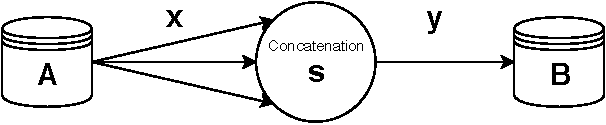
\includegraphics[width=0.48\textwidth]{pics/concat}
  \caption{Strings concatenation physical graph}
  \label{concat}
\end{figure}

\begin{table}[htbp]
\begin {center}
\caption{String concatenation data flow}   \tabcolsep2pt
\begin{tabular}{c|l|c|c|c|c|c|c}      
wall\\ time & $\tau$& $a\in A$  &$x\in W$& $s\in W$ & $y\in W$ & $b \in B$ & step  \\
\hline
1   &   1   &   a   &   a           &           &       &           &   input \\
1   &   2   &   c   &   a,c         &           &       &           &   input \\
1   &   3   &       &    c          &   [a]     &    a  &           &   transform \\
1   &   4   &       &   c           &   [a]     &       &   a       &   output \\
1   &   5   &       &               &   [a,c]   &   ac  &           &   transform \\
1   &   6   &       &               &   [a,c]   &       &   ac       &   output \\
1   &   7   &       &               &   [a,c]   &       &   [a,c]   &   snapshot \\
2   &   8   &   b    &   b          &   [a,c]   &       &           &   input \\
2   &   9   &   d    &   b,d        &   [a,c]   &       &           &   input \\
2   &   10   &       &   b          &   [c,d]   &  cd   &           &   transform \\
2   &   11   &       &   b          &   [c,d]   &       &      cd     &   output \\
2   &   12   &       &              &   [d,b]    &  db   &           &   transform \\
2   &   13   &       &              &   {\bf [d,b]}    &       &      {\bf db}     &   output \\
\arrayrulecolor{red}\hline
3   &   14   &       &               &   [a,c]         &       &           &   recovery \\
3   &   14   &   b   &   b           &   [a,c]         &       &           &   \\
3   &   14   &   d   &   b,d         &   [a,c]         &       &           &   \\
3   &   14   &       &   b           &   [c,d]         &       &           &   \\
3   &   14   &       &   b           &   [c,d]         &       &           &   \\
3   &   14   &       &               &   [d,b]         &       &           &    \\
3   &   14   &       &               &   {\bf [d,b]}   &       &           &    \\
\arrayrulecolor{red}\hline
4   &   15   &  e    &   e           &   [d,b]   &      &           &   input \\
4   &   16   &       &              &   [b,e]   &   be    &          &   transform \\
4   &   17   &       &              &   [b,e]   &       &   {\bf be}       &   output \\
\end{tabular}
\label{concat_example}
\end {center}
\end{table}

\subsection{Model analysis}

In a classical model proposed by Chandy and Lamport~\cite{Chandy:1985:DSD:214451.214456}, a distributed system is represented as a graph of processes, which can be connected via channels. Each process can own a modifiable internal state, generate {\em events} and send them to other processes through the channels. {\em Global system state} in this model contains processes states and channel states, e.g., elements, which are in-flight at the moment. Distributed asynchronous processing is simulated using permutations of events.

The proposed model is a variation of a classical Chandy-Lamport distributed system model with the following properties and modifications:

\begin{itemize}
    \item Our notion of a streaming system does not provide a concept of {\em operations state} because, as it is shown in~\cite{we2018adbis}, states can be considered as common data items. In this case, a state element is presented in a system until it is transformed into a new state together with new elements. This model allows a binary relation $D$ to capture computations within a graph of processes that is a physical streaming execution graph in our case. Hence, the working set $W_\tau$ is a global state with only channel states in terms of Chandy-Lamport.
    \item Input and output elements $a_\tau$ and $b_\tau$ are special events. This way, {\em storage} and {\em computations} are distinguished. We assume that output elements $B_\tau$ are all data that leaves a system including so-called {\em state snapshots} which are typically used for recovery~\cite{Carbone:2017:SMA:3137765.3137777}. Because of this, we state that $X \subseteq W_\tau \cup B_\tau$ in the transform transition of the working set. In most state-of-the-art stream processing systems, the end-user is external to the system, i.e., a user can observe input and output elements, but not the working set.
    \item Distributed asynchronous computations are modeled through the random choice of an operation that is executed next. In the proposed model, instead of using permutations of data flow elements that fixate an execution route, we suppose that the next transition of the working set is a random variable. The distribution of this variable depends on system architecture. 
\end{itemize}

\subsection{Consistency}

The parallel asynchronous nature of distributed stream processing allows us to handle only a {\em probability} of an output element because it can be different from run to run due to element reorderings.

\begin{definition}{Probability of output element}
$P(b_{\tau+1}|A_{\tau}, B_\tau, F)$ is a probability to observe output element $b_{\tau+1}$ considering all previous input and output elements, and recovery function.
\end{definition}

The problem here is that it is hard to define the correct output, because it may significantly vary. Inconsistencies may arise only in case of failure and incorrect recovery. Let us introduce a {\em reference} recovery function that allows us to denote results which are possible to reach without failures.

\begin{definition}{Reference}
$F^{*}$ is a recovery function that restores exactly the same working set as before the failure, $\forall \tau \in \mathbb{N}, F^{*}(A_\tau,B_\tau)=W_\tau$.
\end{definition}

\begin{definition}{Probability of output element with a reference recovery function}
$P(b_{\tau+1}|A_{\tau}, B_\tau, F^{*})$ is a probability to observe output element $b_{\tau+1}$ considering all previous input and output elements, and a reference recovery function.
\end{definition}

Using the notion of a reference recovery function, one can define the correct output. 

\begin{definition}{Output element $b_{\tau+1}$ is consistent}
with all previous input and output elements $A_\tau$ and $B_\tau$ if the probability to observe it is non-zero in a system with reference recovery: $P(b_{\tau+1} \mid A_\tau,B_\tau,F^{*})>0$.
\end{definition}

The reference recovery function allows us to express the notion of correct execution in terms of correspondence between input and output elements. In most real cases, input and output elements are the only data that can be observed by the end-user. In real distributed stream processing systems, failures and recoveries can corrupt the output, despite the fact, that in terms of a simple definition of delivery guarantees, all elements are processed~\eo. 

The problem here is that elements can be concatenated in a different order on recovery. Let us demonstrate it by the already mentioned example demonstrated in Figure~\ref{concat} and Table~\ref{concat_example}. During recovery system may reach concatenation state $s=[b,d]$ at $\tau=15$ rather than $s=[d,b]$ due to asynchronous input. In this case, output at $\tau=17$ becomes {\em de} instead of {\em be}. However, {\em de} is inconsistent with the previous output, because element with prefix {\em d} has already been released at $\tau=13$. It is important to note that all input elements within the example are applied to concatenation state {\em \eo}. This simple example demonstrates that informal definition of\eo\ does not guarantee the consistency of output elements.


% The problem here is that elements can be concatenated in a different order on recovery. This example is shown in Table~\ref{inconsistency_example}. Before the failure, the system reached concatenation state $ "ca" $, but there is no guarantee that a straightforward recovery approach leads to the same state due to asynchronous input. Instead of $"ca"$, state may become $"ac"$. However, output element $ "ca" $ has been already released, and it is expected that the next output starts with the prefix $ "ca" $. It is important to note that even if the next output element is $ "acb" $, that is inconsistent with previously released items, all input elements are applied to concatenation state {\em ~\eo}. This simple example demonstrates that a simple definition of~\eo\ does not guarantee the consistency of output elements.

% \begin{table}[htbp]
% \caption{Output inconsistency due to straightforward recovery}
% \begin{tabular}{cccccc}
% wall time & $\tau$ & $a\in A$ & $W (s=state)$ & $b \in B$ & step  \\
% \hline
% 1 & 1 & $a$ & a & & input    \\
% 1 & 2 & $c$ & $a,c$ &  & input     \\
% 2 & 3 &  & $a,c^{s},c$ &  & transform     \\
% 2 & 4 &  & $a,c^{s}$ & c  & output     \\
% 3 & 5 &  & $ca^{s},ca$ &   & transform     \\
% 3 & 6 &  & $ca^{s}$ & {\bf ca}  & output     \\
% \arrayrulecolor{red}\hline
% 4 & 7 & $a$ & a & & recovery    \\
% 4 & 7 & $c$ & $a,c$ &  &       \\
% 5 & 7 &  & $c,a^{s}$ &  &     \\
% 6 & 7 &  & $ac^{s}$ &   &     \\
% \arrayrulecolor{red}\hline
% 7 & 8 & $b$ & $b,ac^{s}$ &  & input      \\
% 8 & 5 &  & $acb^{s},acb$ &   & transform     \\
% 8 & 6 &  & $acb^{s}$ & {\bf acb}  & output     \\
% \end{tabular}
% \label{inconsistency_example}
% \end{table}

% \begin{table}[htbp]
% \caption{Output inconsistency due to straightforward recovery}
% \begin{tabular}{cccccc}
% wall\\ time & $\tau$ & $a\in A$ & $W$ & $b \in B$ & step  \\
% \hline
% 1 & 1 & $a_{in}$ & $a_{in}$ & & input    \\
% 1 & 2 & $c_{in}$ & $a_{in},c_{in}$ &  & input     \\
% 2 & 3 &  & $a_{in},(c)_{state},(c)_{out}$ &  & transform     \\
% 2 & 4 &  & $a_{in},(c)_{state}$ & $(c)_{out}$  & output     \\
% 3 & 5 &  & $(ca)_{state},(ca)_{out}$ &   & transform     \\
% 3 & 6 &  & $(ca)_{state}$ & $\mathbf{(ca)_{out}}$  & output     \\
% \arrayrulecolor{red}\hline
% 4 & 7 & $a_{in}$ & $a_{in}$ & & recovery    \\
% 4 & 7 & $c_{in}$ & $a_{in},c_{in}$ &  &      \\
% 5 & 7 &  & $c_{in},(a)_{state}$ &  &     \\
% 6 & 7 &  & $(ac)_{state}$ &   &     \\
% \arrayrulecolor{red}\hline
% 7 & 8 & $b_{in}$ & $b_{in},(ac)_{state}$ &  & input      \\
% 9 & 9 &  & $(acb)_{state},(acb)_{out}$ &   & transform     \\
% 9 & 10 &  & $(acb)_{state}$ & $\mathbf{(acb)_{out}}$  & output     \\
% \end{tabular}
% \label{inconsistency_example}
% \end{table}

% Input elements: $"a","b","c","d","e"$

% \begin{table}[htbp]
% \caption{Race effects within multi-class model}
% \begin{tabular}{cc}
%   \\
% \hline
% 2   &   $0.9\pm0.2$    \\
% 4   &   $1.7\pm0.4$    \\
% 8   &   $1.9\pm0.5$    \\
% \end{tabular}
% \label{race_table}
% \end{table}

% Assume that $\Gamma=\mathbb{N}$ and $D$ consists of a single non-commutative operation $v^{i+1}=a_\tau(1+v^{i}),v^{0}=0$ and $v$ becomes an output element on each iteration. The upper index denotes an order of transformations. Let $F$ set $v^{0}=0$ and reprocess input elements from the very beginning that seems like a correct naive approach for restoring. Assume that the system does not release output elements during reprocessing to avoid duplicates. However, if input elements arrive from asynchronous input channels, they can be reordered, and results of non-commutative operation may become inconsistent with results before the failure, e.g., the property of output monotonicity can be violated. This example is demonstrated in Figure~\ref{state-inconsistency}. 

% \begin{figure}[htbp]
%   \centering
%   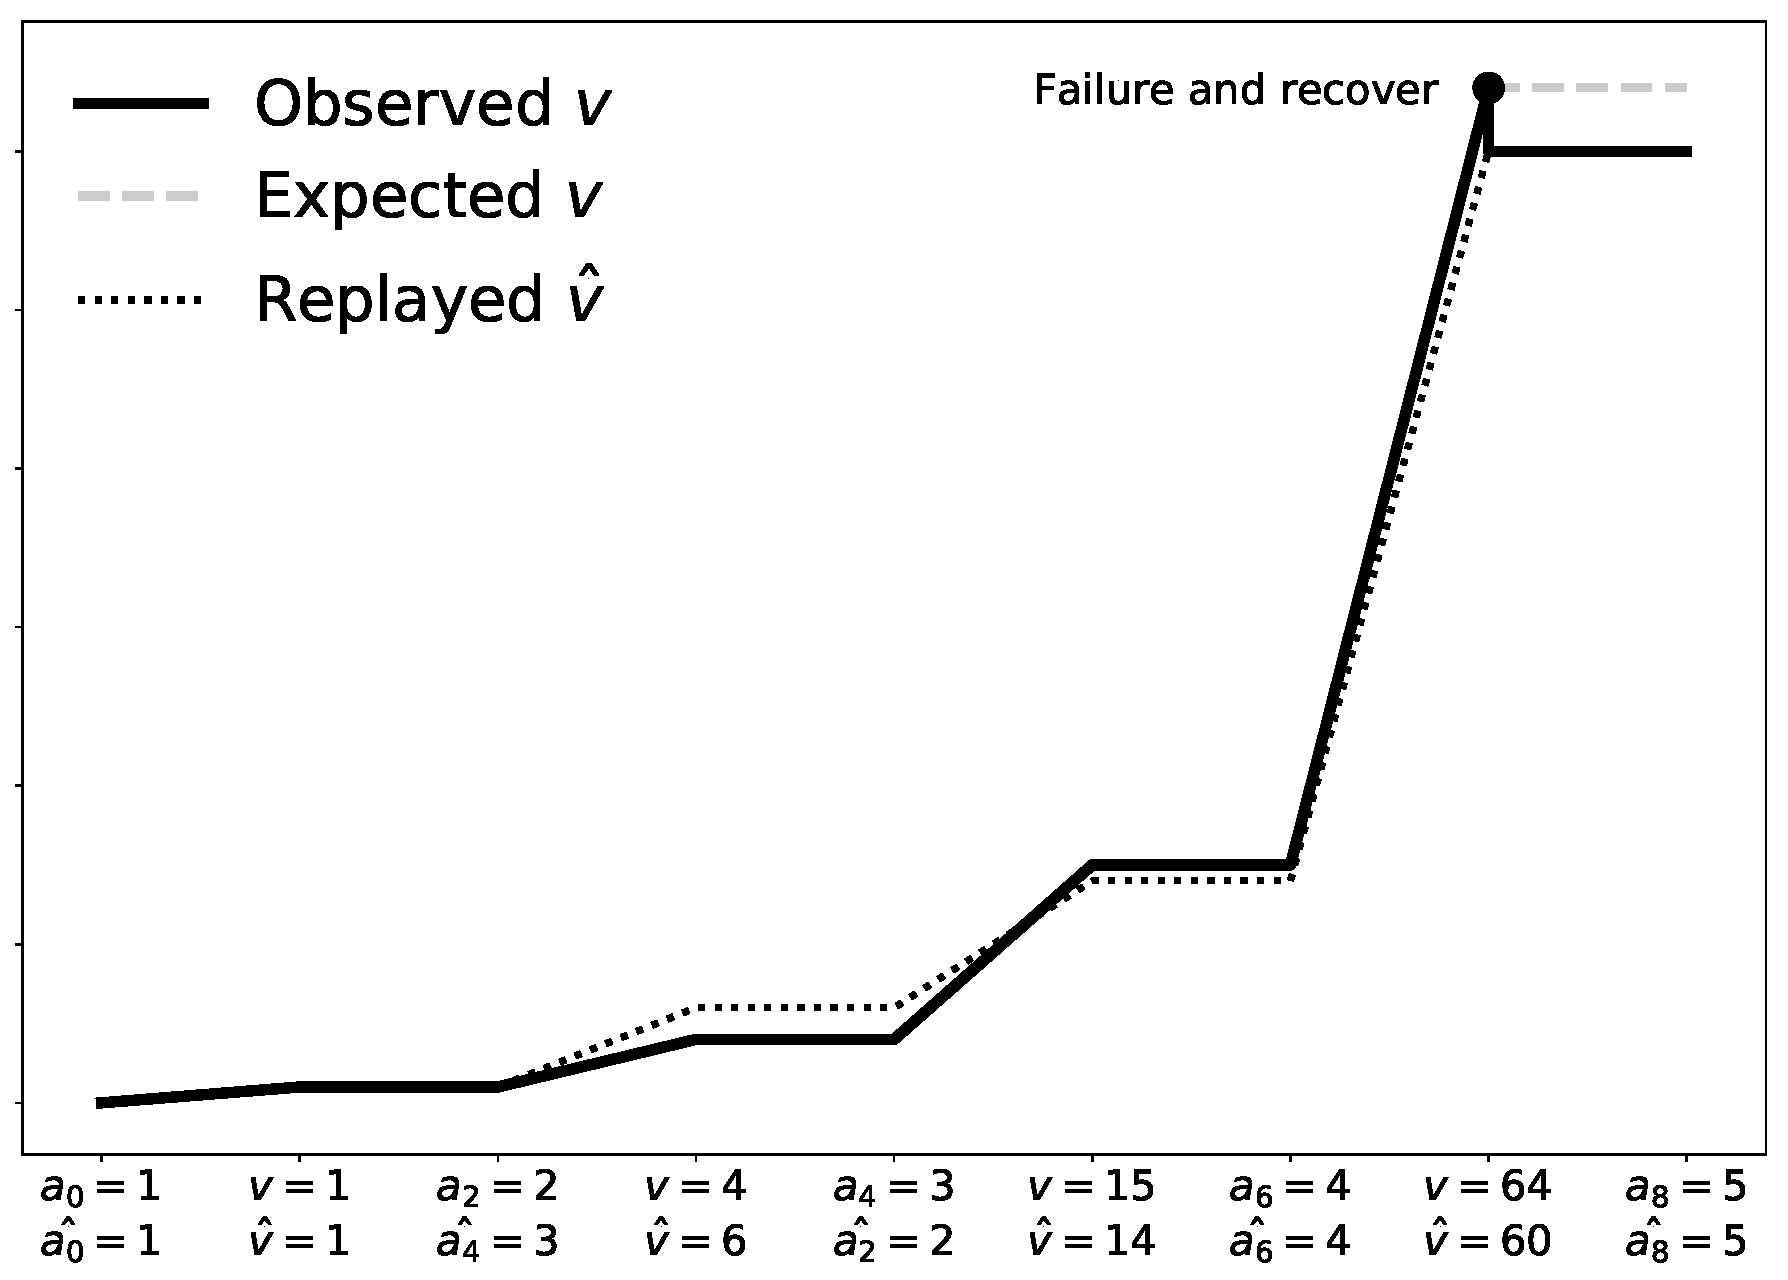
\includegraphics[width=0.48\textwidth]{pics/failure}
%   \caption{Inconsistency of results after complete input reprocessing}
%   \label {state-inconsistency}
% \end{figure}

\subsection{Delivery guarantees}

As we demonstrate further, state-of-the-art stream processing systems prevent inconsistencies illustrated in the example above. However, the informal definition of~\eo\ is insufficient to describe the level of data consistency that is provided. Here we introduce regular definitions of delivery guarantees which take this issue into account. 

\begin{definition}{System provides for~\eo}
if it is possible to obtain each output element $b_{\tau+1}$ in a system with a reference recovery fucntion, i.e.,\\ 
$\forall{\tau \in \mathbb{N}}, b_{\tau+1}\in 2^{\Gamma}: P(b_{\tau+1}|A_{\tau},B_\tau,F)>0 \Rightarrow \\ P(b_{\tau+1}|A_{\tau},B_\tau,F^{*})>0$.
\end{definition}

\begin{definition}{System provides for~\amo}
if \\
$\exists{A^{0}_{\tau}\subseteq{A_{\tau}}}$ such that \\
$\forall{\tau \in \mathbb{N},{b_{\tau+1}\in 2^{\Gamma}}}: P(b_{\tau+1}|A_{\tau},B_\tau,F)>0 \Rightarrow \\ P(b_{\tau+1}|A^{0}_{\tau},B_\tau,F^{*})>0$.
\end{definition}

\begin{definition}{System provides for~\alo}
if \\
$\exists{A^{*}_{\tau}\subseteq{2^{A_{\tau}}}}$ such that \\
$\forall{\tau \in \mathbb{N}, {b_{\tau+1} \in 2^{\Gamma}}}: P(b_{\tau+1}|A_{\tau},B_\tau,F)>0 \Rightarrow \\ P(b_{\tau+1}|A^{*}_{\tau},B_\tau,F^{*})>0$.
\end{definition}

\Eo\ states that observed results cannot be distinguished from one of the possible results produced by a system with a reference recovery function. It means that even if data flow contains races and some elements do not commute, output consistency will be preserved. Looking back to the example illustrated in Table~\ref{concat_example}, our formal definition of~\eo\ ensures that after recovery system reaches state $[d,b]$, not $[b,d]$, because this state has already influenced output elements.

\Amo\ and~\alo\ guarantees are the relaxations of~\eo. The results within these guarantees can be obtained without failures, but with the modification of the input. \Alo\ can be reproduced if the input contains duplicated items. \Amo\ can be achieved with a reference recovery if some input elements are missed. It is important to note, that regarding~\amo\ guarantee we require an input element to be processed atomically with all its derivatives or not processed at all. To the best of our knowledge, none of the stream processing engines supports~\amo\ guarantee, so we cannot verify the relevancy of this assumption. It is accessible to provide~\amo\ by producing no output at all, but if the output is presented,\amo\ enforcement becomes much more difficult.  

In our formal model, the relaxations of~\eo\ are defined without diving into recovery mechanisms. Instead, they are described through possible input channel flaws in a system with a reference recovery. This trick allows us to represent invisible system details in terms clear for an external user.

\subsection{\Eo\ and determinism}

Operations that are presented in $D$ can directly affect the complexity of consistency enforcement mechanisms. For example, if all operations are idempotent, \eo\ can be achieved~\cite{Akidau:2013:MFS:2536222.2536229}. Among common types of operations, non-commutative ones provide significant difficulties in achieving~\eo.

\begin{definition}{D contains non-commutative operation}
if\\ 
$\exists (x,y), s_1, s_2 \in \Gamma, s_1 \neq s_2: \\ ((x,y),s_1)\in D, \\ ((y,x),s_1)\notin D, \\ ((y,x),s_2)\in D$.
\end{definition}

The are many non-commutative operations that are commonly used in practice: concatenation, matrix multiplication, cross product, etc. Hence, general-purpose stream processing systems should support them. The problem with such operations we demonstrated above: simple reprocessing of missing elements in case of failure may lead to results inconsistencies.

\begin{definition}{System is deterministic}
if\\ 
$\forall{\tau\in{\mathbb{N}}, b_{\tau+1}\in{2^{\Gamma}}}:P(b_{\tau+1}|A_{\tau},B_\tau,F^{*})=1$.
\end{definition}

An essential property of a deterministic system is that it preserves the same order of elements before non-commutative operations on each run. We further demonstrate how this property can be used to achieve~\eo\ with low performance overhead.

On the other hand, the absence of determinism imposes restrictions on~\eo\ implementations. The following theorem denotes the necessary and sufficient conditions for~\eo\ in non-deterministic systems with a non-commutative operation in $D$. It demonstrates that if a system is non-deterministic, but supports non-commutative operations, it must save (take a snapshot of) results of non-commutative operations before delivery of output elements that depend on these results.

\begin{figure}[htbp]
  \centering
  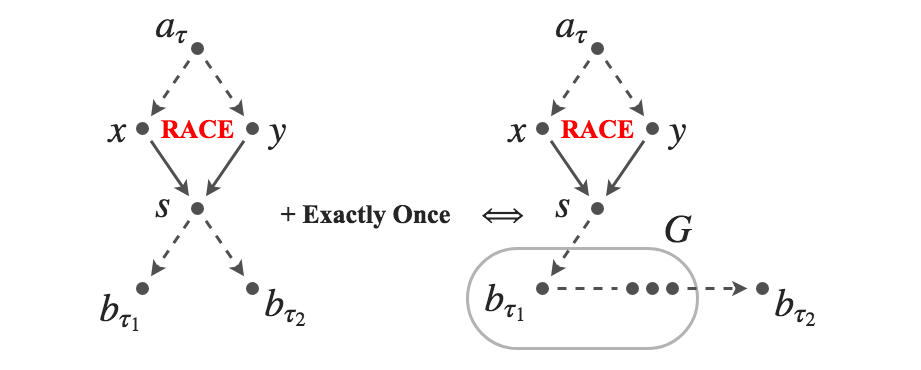
\includegraphics[width=0.48\textwidth]{pics/theorem-pic}
  \caption{The scheme of Theorem~\ref{necessary_conditions}}
  \label {theorem-pic}
\end{figure}

\begin{theorem}
\label{necessary_conditions}
If $D$ contains non-commutative transformation and has the following dependencies for some $a_\tau \in \Gamma$:

\begin{enumerate}
  \item[(i)] $x \in Cl_D(a_\tau), y \in Cl_D(a_\tau)$
  \item[(ii)] $((x,y),s)\in D$ through a non-commutative operation
  \item[(iii)] $b_{\tau_1}, b_{\tau_2} \in Cl_D(s), \tau_1 < \tau_2$
\end{enumerate}

\noindent then non-deterministic system supports~\eo\ if and only if:

\begin{equation}
\label{theorem_conditions}
  \begin{gathered}
    G = Cl_D(b_{\tau_1}) \cap C_D^{-1}(b_{\tau_2}) \\
    \forall (u, v) \in D, u \in Cl_D(s): v \subset G \Rightarrow u \subset G
  \end{gathered}
\end{equation}

\end{theorem}
\begin{sketch}
$ $\newline

The scheme of the theorem is shown in Figure~\ref{theorem-pic}. The theorem conditions mean that each result of the non-commutative operation must become recoverable before the delivery of output that depends on this result. 
% Such behavior is similar to the issue shown in Ta~\ref{state-inconsistency} if we set $b_{\tau_1}=v$.
$ $\newline

\noindent{\em Necessary condition}\newline

  Assume that conditions~\ref{theorem_conditions} are not satisfied, i.e. $\exists v \subset G, u \not\subset G: (u, v) \in D$, and system fails at time $\tau_1<\tau_f<\tau_2$. Then, to obtain $b_{\tau_2}$ there is a need to recompute $v$, $u$ and therefore $s$. However, due to asynchronous distributed processing and non-commutative transformation, system can reach not exactly $s$ such that $((x,y), s) \in D$, but $s':((y,x),s')\in D$. In this case, after recovery element $b_{\tau_2}$ will be delivered, but it will depend not on $s$, but on $s'$: $b_{\tau_2}\in Cl_D(s')$. This is a contradiction, because $b_\tau$ has been already delivered and $P(b_{\tau_2}\in Cl_D(s')|\{a_\tau\},\{b_{\tau_1} \in Cl_D(s) \})=0$.
$ $\newline

\noindent{\em Sufficient condition}
\newline

Let us assume that a  system fails at time $\tau_f$. If $\tau_f < \tau_1$ or $\tau_f > \tau_2$, \eo\ is obviously satisfied. Assume that $\tau_1<\tau_f<\tau_2$. In this case, $b_{\tau_1}\in B_{\tau_f}\subset B_{\tau_2}$. Hence, $b_{\tau_2}$ can be restored directly from $b_{\tau_1}$ without reprocessing of s, i.e. $F(a_\tau,b_{\tau_1})=b_{\tau_2}$ and $b_{\tau_1}, b_{\tau_2} \in Cl_D(s)$ after recovery, thus $P(b_{\tau_2}\in Cl_D(s)|\{a_\tau\},\{b_{\tau_1} \in Cl_D(s) \})>0$.
\end{sketch}


We assume   in this  theorem    that input element $a_\tau$ is split into elements $x,y$. The same behavior can be reproduced if two input elements $a_\tau$ and $a_{\tau+1}$ enter a system through asynchronous channels. In general, this behavior is natural for stream processing systems because elements are processed one-by-one without synchronization and order enforcement. 

This theorem has direct practical implications for non-deterministic systems:
\begin{itemize}
    \item {\bf Output elements must wait until the snapshot is taken}. If a system aims at providing~\eo, it must output elements only if there exists a snapshot that contains results of non-commutative operations. The problem here is that a system is usually not aware of user-defined operations and cannot distinguish commutative and non-commutative operations, so it must wait even if all elements commutate.
    \item {\bf Latency is affected by the period of snapshotting}. The consideration above implies that the lower bound of latency in the worst case in non-deterministic systems is the snapshotting period, together with the duration of taking a snapshot. There is a trade-off between latency and the frequency of taking snapshots because too frequent snapshotting can cause high extra load, while rare snapshots lead to high latency.
\end{itemize}

It is important to note that the proposed model is suitable not only for the formal analysis of the properties of~\eo\ but for a deeper understanding of the other aspects of stream processing. While these topics are promising as well, they are out of the scope of this paper.
